% !TEX root = main.tex

\section{Evaluating the approaches}\label{sec:evaluation}

\subsection{Evaluation methods}

To evaluate and compare the approaches different techniques are used: 
\begin{itemize}
	\item \textbf{K-Fold Cross Validation}: where the data is randomly divided into folds and one of those is used for testing while the rest for training. It is often used in papers containing ML approaches to ranking alerts, though it has its drawbacks. As shown in \cite{performance_method_bug} and as can be seen on \cref{kfold_vs_release}, this approach uses dependent variables (most of the extracted features), that may not be available at prediction time in a real world scenario. That can lead to unreliable and excessively optimistic results. Cross Validation was only used for selecting the right classifier for this task, and not for evaluating the ranking approaches.
	\item \textbf{Release/Revision based testing}: avoids the drawback of the previous method, by using a \textit{"horizontal"} train/test strategy. We fix a certain point in time (revision or release) which defines what the train set (before that point) and test set (after that point) will be. This trains the algorithms with more realistic data, but it also has its drawbacks. In a scenario where the dataset is imbalanced, a \textit{"horizontal"} 80/20\% split may leave us with very little data. Also, unlike in cross validation, we cannot train and test different models.
	
	\begin{figure}[H]
		\centering
		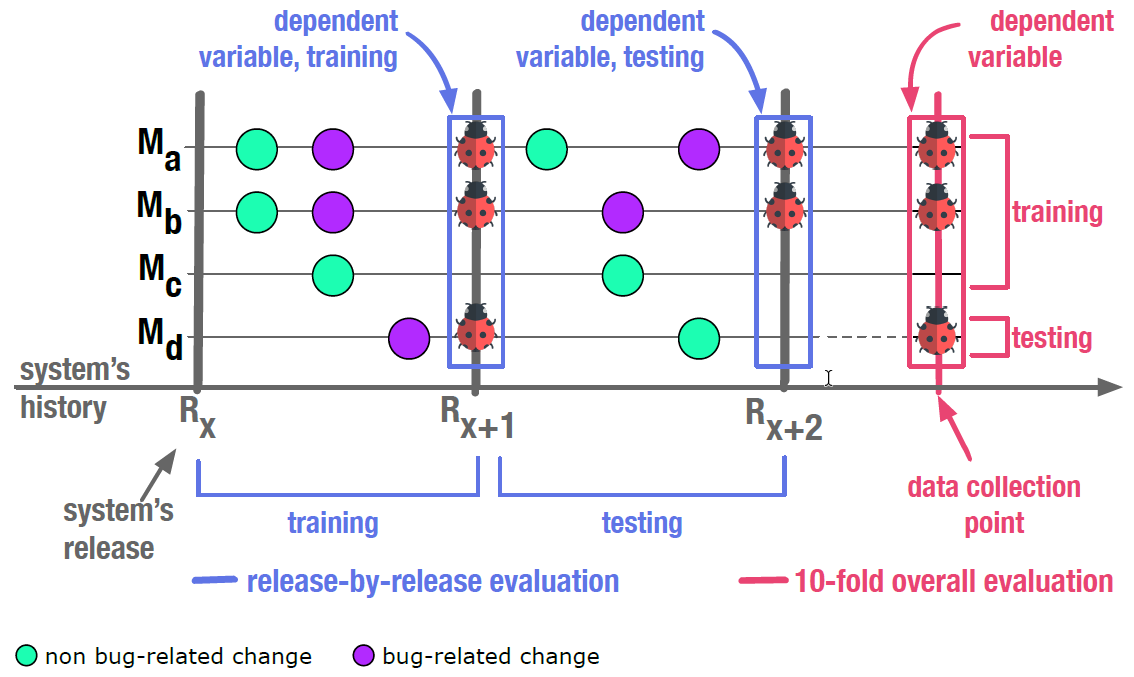
\includegraphics[scale=0.3]{./src/release_based_testing.png}
		\caption{Release-based vs K-Fold (\cite{performance_method_bug})}
		\label{kfold_vs_release}
	\end{figure}
	
	\item \textbf{Average FP to TP \cite{correlation_exploitation}}: Let N be the total number of actionable alerts in a set of reports, and $FP_j$ is the number of false positives to inspect for finding the \textit{j}th actionable alert, starting from the last actionable alert inspected. Formula~\ref{eq:avg-fp-tp} defines the Average FP to TP.
	
	\begin{equation} \label{eq:avg-fp-tp}
		\mathit{AVG_{FP-TP}}(R) = \frac{\sum_{i=1}^{N} FP_j}{N}
	\end{equation}

	
	\item \textbf{Z-Ranking Score - S(R) \cite{z-ranking}:} 
Let \textit{N} be the total number of alerts and \textit{act} the number of actionable ones. Let \textit{R(i)} denote the cumulative number of actionable alerts found by a ranking scheme \textit{R} on the \textit{i}th inspection. We show how to measure the Z-Ranking Score in Formula~\ref{eq:score}.

	\begin{equation} \label{eq:score}
	S(R) = \sum_{i=1}^{N} [\mathit{min}(i,\mathit{act}) - R(i)]
	\end{equation}
	\item \textbf{Comparison against random rankings}: where we compare if the ranking produced by a model is better than a random order of alerts. We calculate that by using the two previously defined metrics, Average FP to TP and S(R).
	Also we compare the number of actionable alerts found in the first \textit{X} places in a ranked list, compared to a random list.
	\item \textbf{Cumulative ranking graph}: formed by plotting the number of actionable alerts found within the first N inspections.
\end{itemize}

\subsection{Evaluation Metrics}

Along with the classic evaluation metrics like \textit{accuracy}, \textit{precision} and \textit{recall}, other metrics are used that are more appropriate for imbalanced data \cite{comparison_metrics, iba_metric}. 
Sensitivity, or True Positive Rate is the percentage of positive examples which
are correctly classified (Formula~\ref{eq:sensitivity}).
Specificity, or True Negative Rate, is the percentage of negative examples which are correctly classified (Formula~\ref{eq:specificity}).
G-Mean is the geometric mean of the sensitivity and specificity (Formula~\ref{eq:g-mean}).


\begin{equation} \label{eq:sensitivity}
\mathit{Sensitivity} = \frac{TP}{TP + FN}
\end{equation}

\begin{equation} \label{eq:specificity}
\mathit{Specificity} = \frac{TN}{FP + TN}\\
\end{equation}

\begin{equation} \label{eq:g-mean}
G{\text -}\mathit{Mean} = \sqrt{ \mathit{Sensitivity} * \mathit{Specificity}}
\end{equation}

The \textit{AUC} of a binary classifier is equivalent to the probability that the classifier will rank a randomly chosen positive instance higher than a randomly chosen negative instance. We are using the approximation formula for \textit{AUC} according to the trapezoid rule (Formula~\ref{eq:auc}).

\begin{equation} \label{eq:auc}
\mathit{AUC} = \frac{\mathit{Sensitivity} + \mathit{Specificity}}{2} 
\end{equation} 

The \textit{Index of Balanced Accuracy} used for evaluating learning processes in two-class imbalanced domains. The
method combines an unbiased index of its overall accuracy and a measure about
how dominant is the class with the highest individual accuracy rate (Formula~\ref{eq:iba}).

\begin{equation} \label{eq:iba}
\mathit{IBA_{\alpha}} = (1 + \alpha * (\mathit{Sensitivity} - \mathit{Specificity})) * \mathit{Sensitivity} * \mathit{Specificity}
\end{equation} 


%\subsubsection{Preparing the dataset}
%\textbf{TODO: EVALUATE ENCODING METHODS}

\subsection{Results of the approaches}

We run the experiments by training methods on the first 80\% items of the dataset and testing on the remaining 20\%.
\henrique{By using Cross Validation or Release/Revision testing? It is important to highlight here again.}

For the actionable alert (\cref{method:actalerts}) and method bug prediction (\cref{method:bugprediction}) approaches, we considered three different classifiers. We chose the classifiers based on the nature of the data (categorical variables, ordinal, discrete values) and the state of the art in the field: \textit{Random Forest}, \textit{AdaBoost}, and \textit{LightGBM}.

To decide between the three, a 10-fold validation was performed and timed in a subset of the data. \textit{LightGBM} was finally chosen because of the good performance and speed (\textit{AdaBoost} does not support multi-threading in the \textit{scikit} library).
The results can be seen on \cref{choosing_classifier}.

\begin{longtable}[c]{@{}lcccr@{}}
	\caption{Classifier performance on a 10-fold validation on actionable alerts}
	\label{choosing_classifier}\\
	\toprule
	& Precision & Recall & Accuracy & Time  \\* \midrule
	\endfirsthead
	%
	\endhead
	%
	\bottomrule
	\endfoot
	%
	\endlastfoot
	%
	Random Forest (30 threads) & 89        & 97     & 90       & 14.8s \\
	LightGBM (30 threads)      & 98        & 93     & 94       & 9.1s  \\
	AdaBoost      & 96        & 94     & 94       & 89.0s   \\* \bottomrule
\end{longtable}


In order to evaluate the ranking, two metrics are used to compare the ranked alerts with a random order (\textit{S(R)} and \textit{Average FP-to-TP}). The experiments are run multiple times (by shuffling the random order and calculating the metrics again). Also the number of valuable alerts in the top \textit{X} places of the improved ranking is compared against random ranking. \henrique{How many times exactly did you run the experiments? (yes this is important). Moreover, how did you select the metric when you run multiple times? Or did you compute the average, or median?}


\subsubsection{Actionable Alerts}
\label{results:actionable_alerts}

Alerts are ranked based on the probabiliy score produced by the classifier for the prediction target (actionable or not). \henrique{I am a little confused here. The section is about actionable alerts but in the first sentence you state the alerts are ranked for the predcition actionable or not. Then how are you measuring actionable alerts?}

As can be seen on \cref{result:actalerts}, the choice of the balancing technique or cleaning method has little impact on the metrics (they are quite good for each case). The best performing one is \textit{ADASYN} (\cref{results:actalerts_best}.) \henrique{Are you sure about these results? If the random sample has a f-score of 95\%, I do not see much gain with other techniques with 96\%. Moreover, a two percent different among techniques may be statiscally insignificant.}

The order produced by the \textit{LightGBM} classifier always outperforms the random order and it also contains around 50\% more actionable alerts in the top 100 or 1000 places (\cref{results:ranking_actalerts}).

Furthermore, as can be seen on the cumulative graph on \cref{results:cumulative_actalerts}, the order of the ranked alerts is close to perfect.

\begin{table}[H]
	\caption{Results of different cleaning and balancing methods for the Actionable Alerts approach}
	\label{result:actalerts}
	\centering
	\begin{tabular}{@{}ccccccc@{}}
		\toprule
		& \textbf{Precision} & \textbf{Recall} & \textbf{Specificity} & \textbf{F1-Score} & \textbf{Geometric} & \textbf{IBA}  \\ \midrule
		\textit{Random Over Sampler}             & 94\%               & 93\%            & 95\%                 & 93\%              & 94\%               & 88\%          \\
		\textit{Random Under Sampler}            & 95\%               & 94\%            & 96\%                 & 95\%              & 95\%               & 90\%          \\
		\textit{SMOTE}                           & 94\%               & 94\%            & 96\%                 & 94\%              & 95\%               & 89\%          \\
		\textit{ADASYN}                          & \textbf{97\%}      & \textbf{97\%}   & \textbf{98\%}        & \textbf{97\%}     & \textbf{98\%}      & \textbf{95\%} \\
		\textit{SMOTEENN}                        & 94\%               & 94\%            & 96\%                 & 94\%              & 95\%               & 90\%          \\
		\textit{SMOTETomek}                      & 95\%               & 94\%            & 96\%                 & 94\%              & 95\%               & 90\%          \\
		\textit{EditedNearestNeighbours}         & 95\%               & 94\%            & 96\%                 & 94\%              & 95\%               & 90\%          \\
		\textit{RepeatedEditedNearestNeighbours} & 95\%               & 95\%            & 96\%                 & 95\%              & 96\%               & 91\%          \\
		\textit{AllKNN}                          & 95\%               & 95\%            & 96\%                 & 95\%              & 96\%               & 91\%          \\
		\textit{OneSidedSelection}               & 95\%               & 94\%            & 96\%                 & 94\%              & 95\%               & 90\%          \\
		\textit{NeighbourhoodCleaningRule}       & 95\%               & 95\%            & 96\%                 & 95\%              & 95\%               & 90\%          \\ \bottomrule
	\end{tabular}
	\textit{Calculated using the balanced classification report of \textit{imblearn} \cite{imblearn}}
\end{table}

\begin{figure}[H]
	\begin{subfigure}{\textwidth}
		\centering
		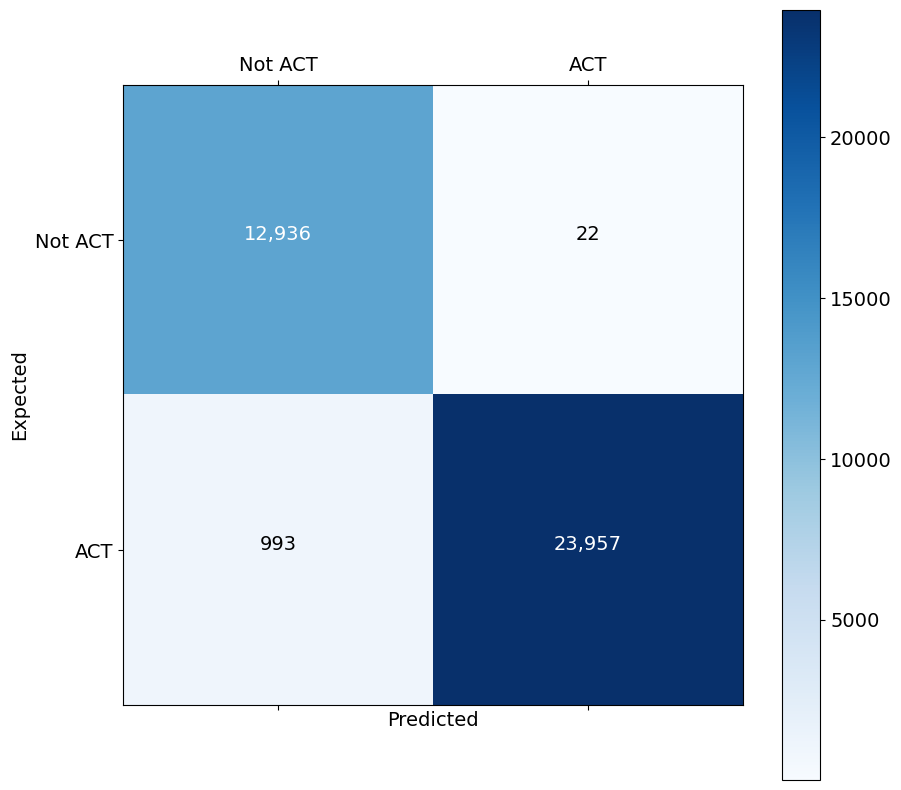
\includegraphics[scale=0.3]{./src/actAlerts/actalerts_adasyn_cm.png}
		\caption{Confusion matrix}\label{}
	\end{subfigure}\\
	\begin{subfigure}{.5\textwidth}
		\centering
		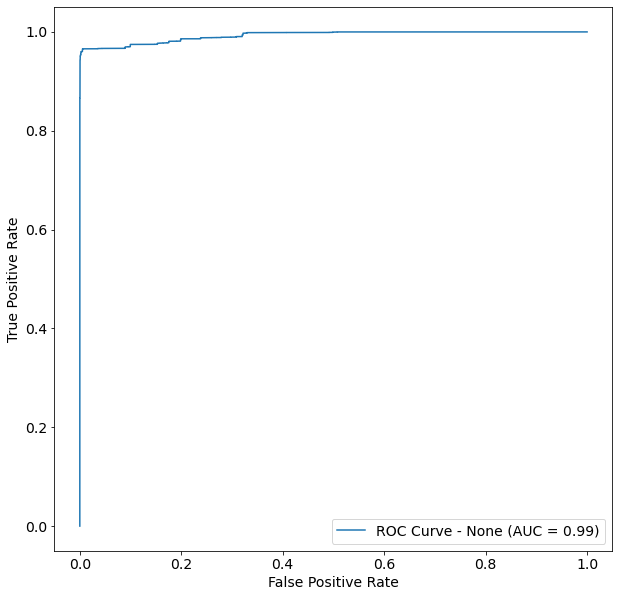
\includegraphics[scale=0.3]{./src/actAlerts/actalerts_adasyn_roc.png}
		\caption{ROC Curve}\label{}
	\end{subfigure}%
	\begin{subfigure}{.5\textwidth}
		\centering
		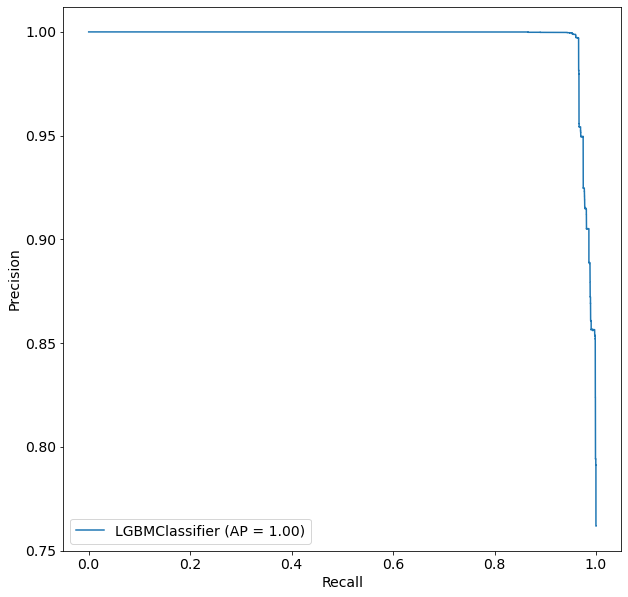
\includegraphics[scale=0.3]{./src/actAlerts/actalerts_adasyn_pr.png}
		\caption{Precision/Recall curve}\label{}
	\end{subfigure}  
	\caption{Actionable alerts with ADASYN}
	\label{results:actalerts_best}
\end{figure}

\begin{table}[H]
	\caption{Comparison against random ranking for the Actionable Alerts approach}
	\label{results:ranking_actalerts}
	\centering
	\begin{tabular}{@{}lccc@{}}
		\toprule
		& \textbf{S(R) metric}  & \textbf{Average FP to TP} & \textbf{Number Actionable}    \\ \midrule
		\textit{Better than random Top 100 alerts}  & 1000 out of 1000 runs & 1000 out of 1000          & 52\% more than random ranking \\
		\textit{Better than random Top 1000 alerts} & 1000 out of 1000 runs & 1000 out of 1000          & 51\% more than random ranking \\
		\textit{Better than random All alerts}      & 10 out of 10 runs     & 10 out of 10              & \multicolumn{1}{l}{}          \\ \bottomrule
	\end{tabular}
\end{table}

\begin{figure}[H]
	\centering
	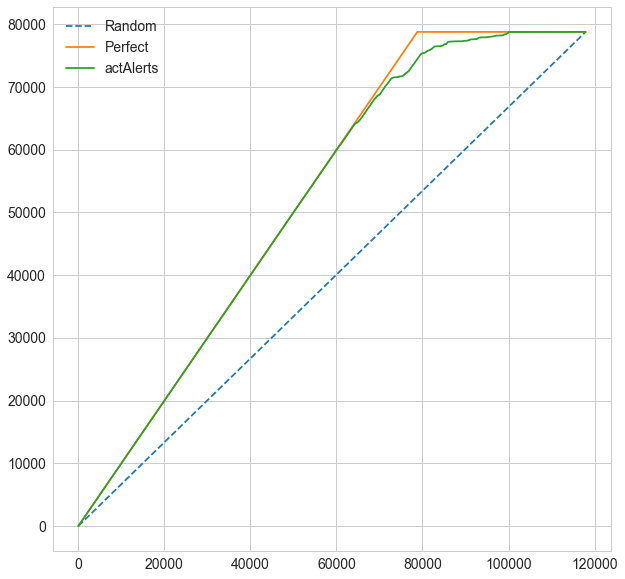
\includegraphics[scale=0.4]{./src/actAlerts/cumulative_graph_all.png}
	\caption{Cumulative ranking graph for Actionable Alerts}
	\label{results:cumulative_actalerts}
\end{figure}


\subsection{Method Bug Prediction}

The overall results for predicting if a method will be buggy in the future, are far from optimal. Predicting bugs on a finer granularity is a hard task, but for the purpose of our use, prioritizing alerts on methods with a higher probability of being buggy, the actual achieved performance can still be regarded as a good starting point.
As can be seen on \cref{result:bugPrediction}, the choice of the balancing technique or cleaning method has a clear impact on some the metrics. The best performing one is \textit{One Sided Selection} (\cref{results:bugprediction_best}). 

Even though the main purpose of this method is not to detect actionable alerts in general, but to give extra attention to alerts belonging to buggy methods, we conduct an experiment to see if we can rank actionable alerts by using the probability of a method being buggy.

Having calculated the set of buggy methods, we can also explore if there is a correlation between the amount of alerts of a particular category/type and the method being buggy. As can be noticed on \cref{results:buggy_correlationss}, the amount of correlation is limited. 

After calculating the probability of a method being buggy on the test set, we merge that set with the one containing actionable alerts (thus only those alerts that are located on the methods in the test set). Alerts are ranked based on the probability score produced by the classifier for the prediction target (buggy method or not). %The goal is to see if ranking alerts higher when they belong to a bug prone method is useful in terms of predicting if that alert will be actionable in the future.

Alerts ranked by bug-prone method probability outperform the random order in the first 100 and 1000 alerts, but not on the whole dataset (\cref{results:ranking_methodbug_alerts}).

On the cumulative graphs we can see that until the first 2000 alerts, the improved ranking significantly outperforms the random one (\cref{results:cumulative_bugprediction}).

From the results we can conclude that ranking alerts based on the method being bug-prone provides an improvement against the random order. \henrique{If you concluded something here, it should appear in your conclusion.}

\begin{table}[H]
	\caption{Results of different cleaning and balancing methods for the Method Bug Prediction approach}
	\label{result:bugPrediction}
	\centering
	\begin{tabular}{@{}ccccccc@{}}
		\toprule
		& \textbf{Precision} & \textbf{Recall} & \textbf{Specificity} & \textbf{F1-Score} & \textbf{Geometric} & \textbf{IBA}  \\ \midrule
		\textit{Random Over Sampler}             & 64\%               & 71\%            & 34\%                 & 65\%              & 33\%               & 11\%          \\
		\textit{Random Under Sampler}            & 67\%               & 72\%            & 36\%                 & 66\%              & 37\%               & 14\%          \\
		\textit{SMOTE}                           & 66\%               & 72\%            & 35\%                 & 66\%              & 35\%               & 13\%          \\
		\textit{ADASYN}                          & 66\%               & 72\%            & 34\%                 & 65\%              & 32\%               & 11\%          \\
		\textit{SMOTEENN}                        & 64\%               & 71\%            & 33\%                 & 64\%              & 30\%               & 10\%          \\
		\textit{SMOTETomek}                      & 66\%               & 72\%            & 36\%                 & 66\%              & 37\%               & 14\%          \\
		\textit{EditedNearestNeighbours}         & 68\%               & 70\%            & 45\%                 & 68\%              & 51\%               & 26\%          \\
		\textit{RepeatedEditedNearestNeighbours} & 68\%               & 71\%            & 45\%                 & 69\%              & 51\%               & 27\%          \\
		\textit{AllKNN}                          & 68\%               & 71\%            & 46\%                 & 69\%              & 52\%               & 27\%          \\
		\textit{OneSidedSelection}               & \textbf{71\%}      & \textbf{72\%}   & \textbf{54\%}        & \textbf{72\%}     & \textbf{60\%}      & \textbf{37\%} \\
		\textit{NeighbourhoodCleaningRule}       & 69\%               & 72\%            & 47\%                 & 70\%              & 53\%               & 28\%          \\ \bottomrule
	\end{tabular}
	\textit{Calculated using the balanced classification report of \textit{imblearn} \cite{imblearn}}
\end{table}

\begin{figure}[H]
	\begin{subfigure}{\textwidth}
		\centering
		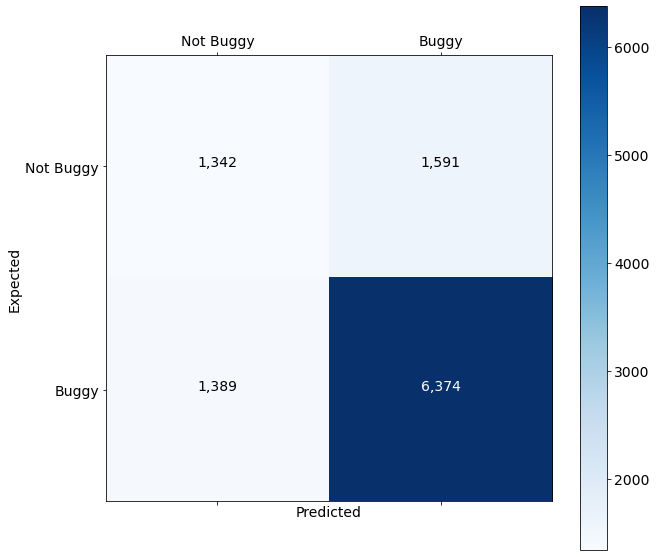
\includegraphics[scale=0.3]{./src/methodBug/methodbug_onesidedselection_cm.png}
		\caption{Confusion matrix}\label{}
	\end{subfigure}\\
	\begin{subfigure}{.5\textwidth}
		\centering
		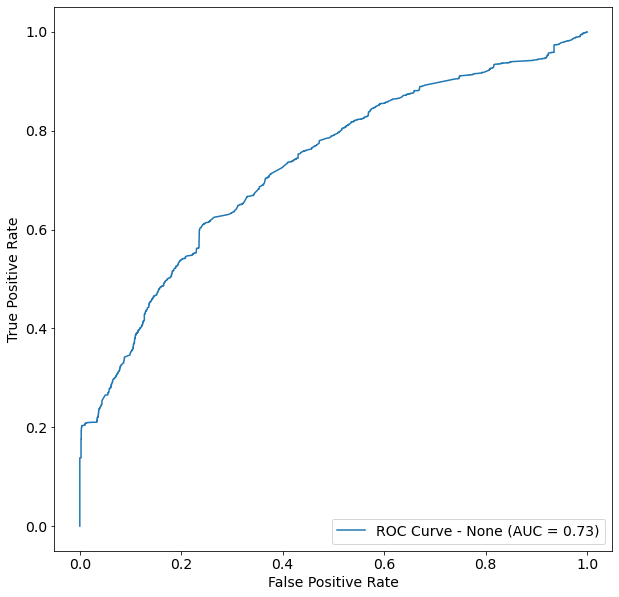
\includegraphics[scale=0.3]{./src/methodBug/methodbug_onesidedselection_roc.png}
		\caption{ROC Curve}\label{}
	\end{subfigure}%
	\begin{subfigure}{.5\textwidth}
		\centering
		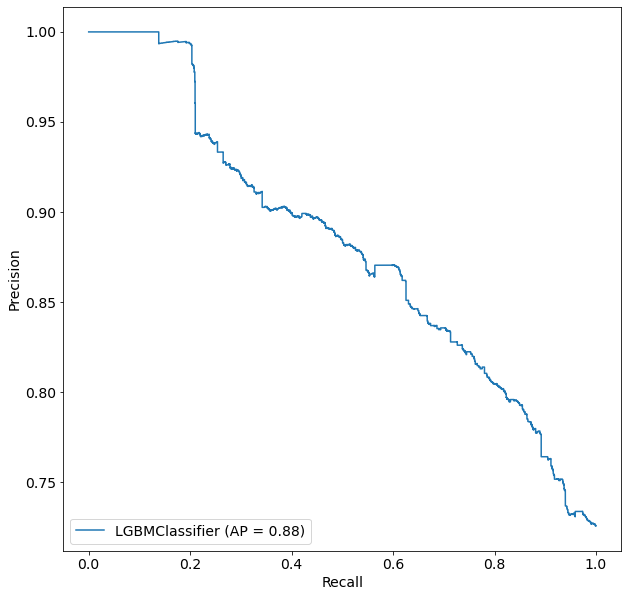
\includegraphics[scale=0.3]{./src/methodBug/methodbug_onesidedselection_pr.png}
		\caption{Precision/Recall curve}\label{}
	\end{subfigure}  
	\caption{Method Bug Prediction with One Sided Selection}
	\label{results:bugprediction_best}
\end{figure}


\begin{figure}[H]
	\begin{subfigure}{\textwidth}
		\centering
		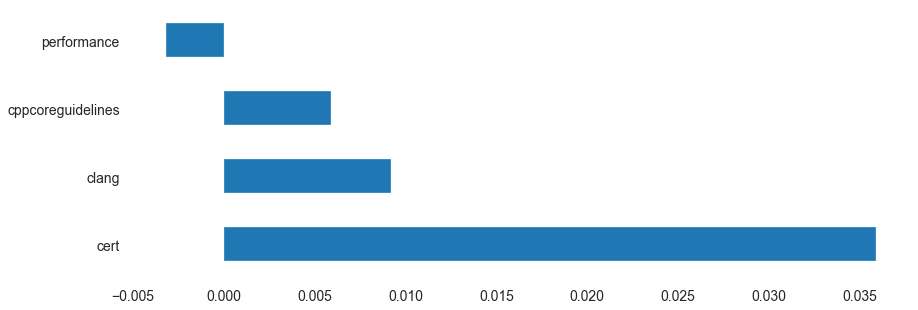
\includegraphics[scale=0.3]{./src/methodBug/methodbug_category_correlations.png}
		\caption{Category correlations}\label{}
	\end{subfigure}\\
	\begin{subfigure}{\textwidth}
	\centering
	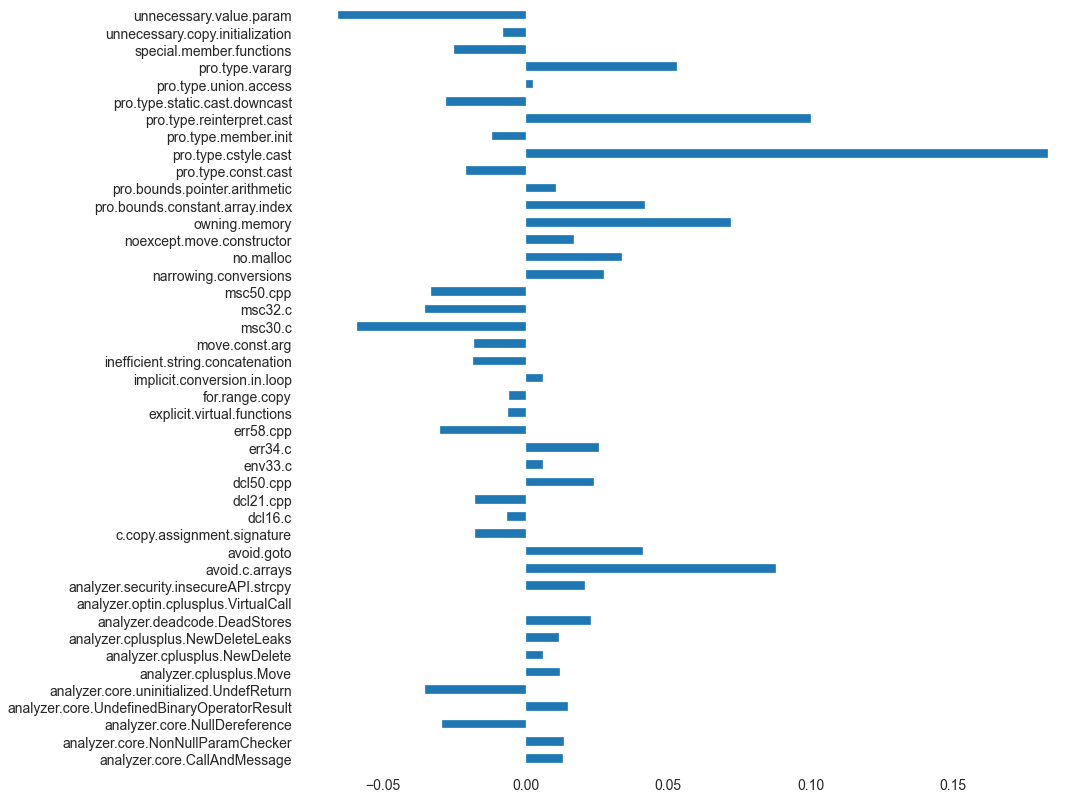
\includegraphics[scale=0.3]{./src/methodBug/methodbug_type_correlations.png}
	\caption{Type correlations}\label{}
	\end{subfigure}
	\caption{Correlation of buggy methods with closed alerts}
	\label{results:buggy_correlationss}
\end{figure}


\begin{table}[H]
	\caption{Comparison against random ranking for the Method Bug Prediction approach}
	\label{results:ranking_methodbug_alerts}
	\centering
	\begin{tabular}{@{}lccc@{}}
		\toprule
		& \textbf{S(R) metric}  & \textbf{Average FP to TP} & \textbf{Number Actionable}    \\ \midrule
		\textit{Better than random Top 100 alerts}  & 1000 out of 1000 runs & 1000 out of 1000          & 75\% more than random ranking \\
		\textit{Better than random Top 1000 alerts} & 1000 out of 1000 runs & 1000 out of 1000          & 57\% more than random ranking \\
		\textit{Better than random All alerts}      & 0 out of 10 runs      & 9 out of 10               & \multicolumn{1}{l}{}          \\ \bottomrule
	\end{tabular}
\end{table}

\begin{figure}[H]
	\begin{subfigure}{\textwidth}
		\centering
		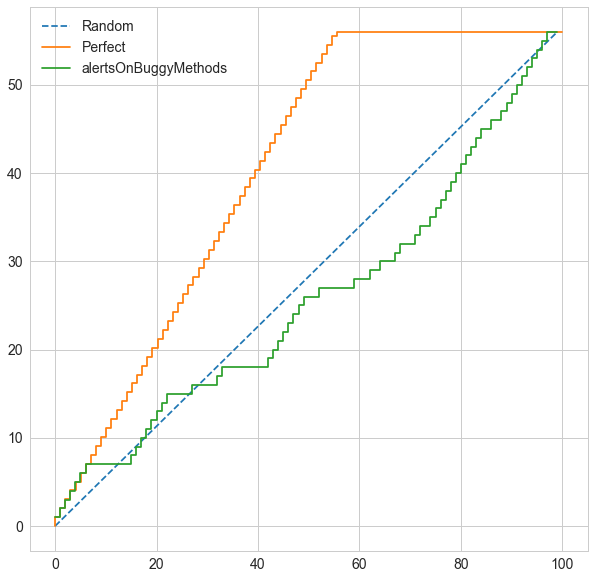
\includegraphics[scale=0.3]{./src/methodBug/methodbug_cumulative_graph_top100.png}
		\caption{Top 100 alerts}\label{}
	\end{subfigure}\\
	\begin{subfigure}{.5\textwidth}
		\centering
		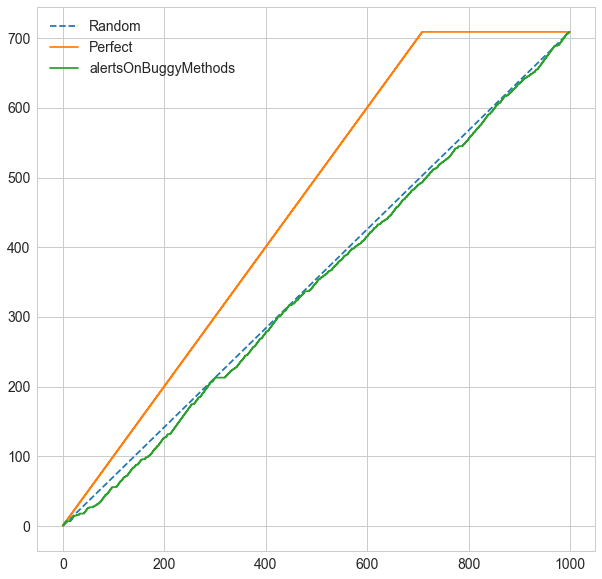
\includegraphics[scale=0.3]{./src/methodBug/methodbug_cumulative_graph_top1000.png}
		\caption{Top 1000 alerts}\label{}
	\end{subfigure}%
	\begin{subfigure}{.5\textwidth}
		\centering
		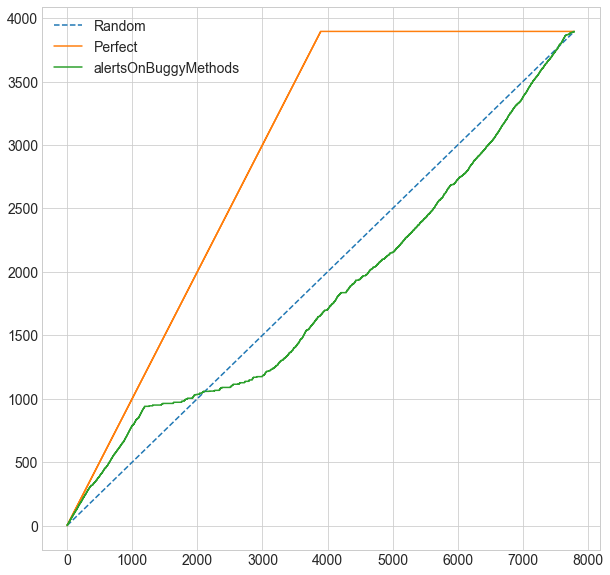
\includegraphics[scale=0.3]{./src/methodBug/methodbug_cumulative_graph_all.png}
		\caption{All alerts}\label{}
	\end{subfigure}
	\caption{Cumulative ranking graph for Method Bug Prediction}
	\label{results:cumulative_bugprediction}
\end{figure}

\subsection{Feedback Rank}

These experiments were run on a small subset of the dataset. The Bayes Network was trained on 10,000 samples and tested on 1,000. The reason being the abnormally high runtime (one hour to predict 1,000 warnings). That could be explained by the size of the network, given that our project has hundreds of packages and thousands of files and methods.

Different balancing algorithms were applied to the training set and \textit{Bayes Network} was used as a classifier (\cref{result:fbrank}). Random over sampling seems to perform the best, but the overall results are rather poor (\cref{results:metrics_fbrank}).

Alerts were ranked according to the probability produced by the Bayes Network. Based on the top 100 results, Feedback Rank performs even worse than random ranking, while doing better on the whole 1000 alert set (\cref{results:ranking_fbrank}, \cref{results:cumulative_fbrank}).

\begin{table}[H]
	\caption{Results of different balancing methods for the Feedback Rank approach}
	\label{result:fbrank}
	\centering
	\begin{tabular}{@{}ccccccc@{}}
		\toprule
		& \textbf{Precision} & \textbf{Recall} & \textbf{Specificity} & \textbf{F1-Score} & \textbf{Geometric} & \textbf{IBA}  \\ \midrule
		\textit{Random Under Sampler}  & 57\%               & 55\%            & 57\%                 & 52\%              & 51\%               & 26\%          \\
		\textit{Random Over Sampler} & \textbf{61\%}      & \textbf{58\%}   & \textbf{60\%}        & \textbf{56\%}     & \textbf{55\%}      & \textbf{30\%} \\
		\textit{None}                 & 59\%               & 56\%            & 58\%                 & 53\%              & 51\%               & 26\%          \\ \bottomrule
	\end{tabular}

	\textit{Calculated using the balanced classification report of \textit{imblearn} \cite{imblearn}}
\end{table}


\begin{figure}[H]
	\begin{subfigure}{0.5\textwidth}
		\centering
		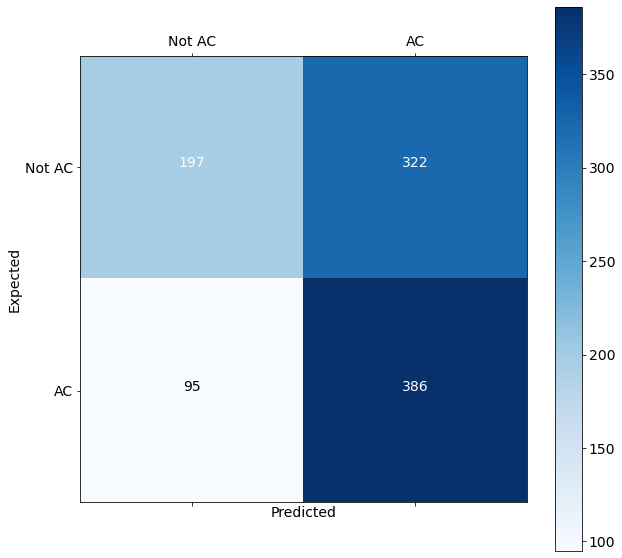
\includegraphics[scale=0.3]{./src/fbRank/fbrank_ro_cm.png}
		\caption{Confusion matrix of test set for unbalanced training set}\label{}
	\end{subfigure}%
	\begin{subfigure}{0.5\textwidth}
	\centering
	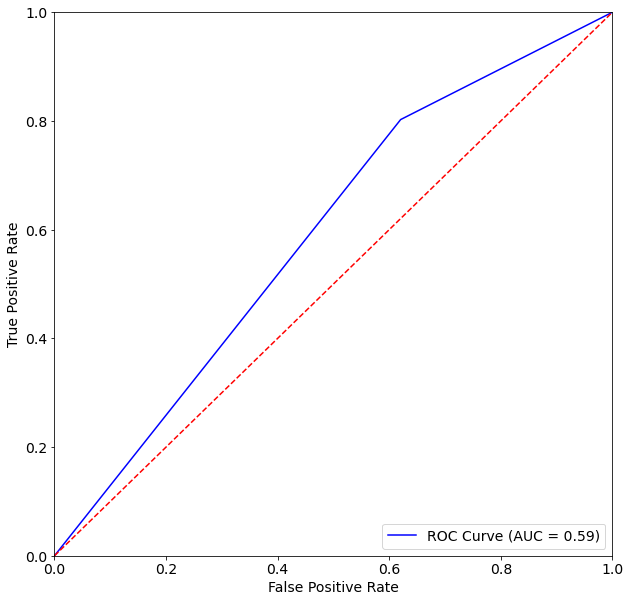
\includegraphics[scale=0.28]{./src/fbRank/fbrank_ro_roc.png}
	\caption{ROC Curve}\label{}
	\end{subfigure}
	\caption{Feedback Rank with Random Over Sampling}
	\label{results:metrics_fbrank}
\end{figure}

\begin{table}[H]
	\caption{Comparison against random ranking for the Feedback Rank approach}
	\label{results:ranking_fbrank}
	\centering
	\begin{tabular}{@{}lccc@{}}
		\toprule
		& \textbf{S(R) metric}  & \textbf{Average FP to TP} & \textbf{Number Actionable}    \\ \midrule
		\textit{Better than random Top 100 alerts}  & 0 out of 1000 runs    & 85 out of 1000            & 13\% less than random ranking \\
		\textit{Better than random Top 1000 alerts} & 1000 out of 1000 runs & 869 out of 1000           &                               \\ \bottomrule
	\end{tabular}
\end{table}

\begin{figure}[H]
	\begin{subfigure}{.5\textwidth}
		\centering
		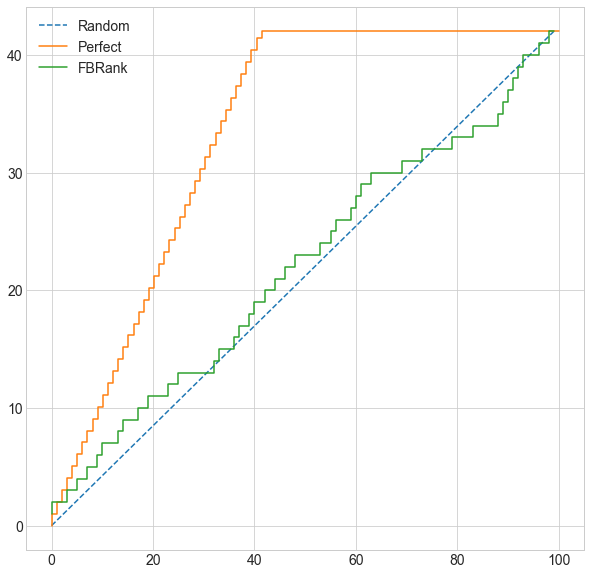
\includegraphics[scale=0.3]{./src/fbRank/fbrank_cumulative_graph_top100.png}
		\caption{Top 100 alerts}\label{}
	\end{subfigure}%
	\begin{subfigure}{.5\textwidth}
		\centering
		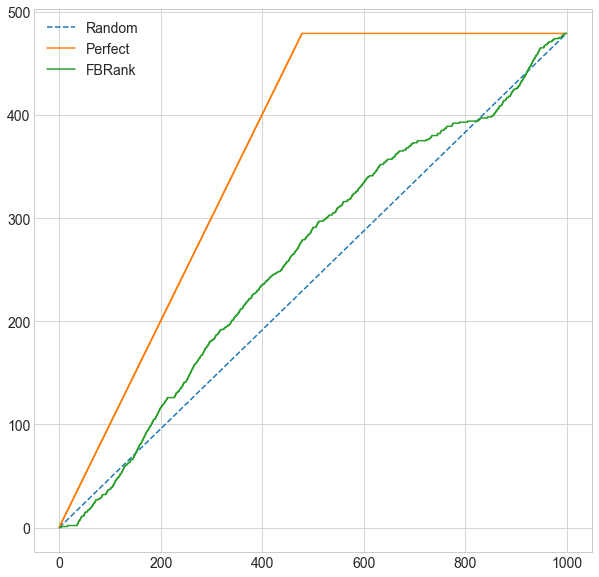
\includegraphics[scale=0.3]{./src/fbRank/fbrank_cumulative_graph_top1000.png}
		\caption{Top 1000 alerts}\label{}
	\end{subfigure}
	\caption{Cumulative ranking graph for Feedback Rank}
	\label{results:cumulative_fbrank}
\end{figure}


\subsection{Bug-Related Lines}

By analyzing the bug-fix revision we are able to collect around 8,700 bug-related alerts (alerts pointing to a bug-related line or method). The type and category distribution of these alerts can be seen on \cref{results:bralerts}

Since this method only calculates weights for alert types, it does not predict if a particular alert is actionable or not. As a consequence, only the ranking is evaluated and not the other metrics.

In contrast to previous methods, the train and test set was split equally (gave better results). \henrique{By using Cross Validation or Released/Revision? Moreover, why this split gives better results?}

The algorithm ranks alerts types based on two input weight parameters ($\alpha,\beta$). Based on experimental evaluation the following respective values were chosen: $\alpha=0.7, 
\beta=0.3$. \henrique{How did you conduct this experimental evaluation to discover these values? Trying values at random is not 'experimental evaluation'. Experimental evaluation implies a method or at least some structure.}
The particular value of these variables did not make much difference on the experiment results, rather than if of them is bigger than the other.
\henrique{If the values did not make much difference, then why the experimental evaluation to find which ones to use? Are the difference statistically insignificant?}

As can be seen from \cref{results:ranking_brls} and \cref{results:cumulative_brls} the algorithms performs well both on the top 100 and 1,000 alerts.

\begin{figure}[H]
	\begin{subfigure}{0.5\textwidth}
		\centering
		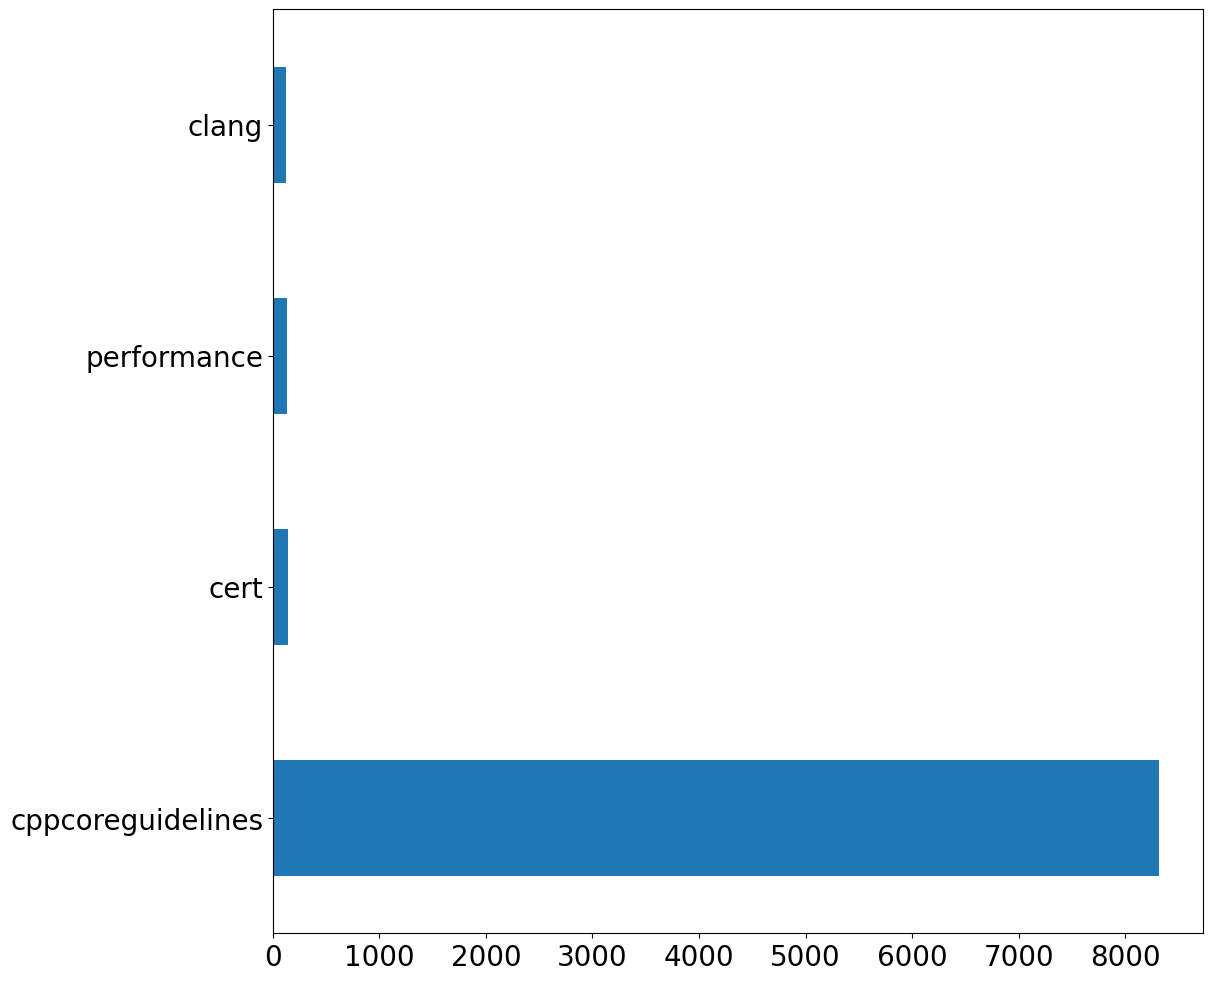
\includegraphics[scale=0.24]{./src/brls/brls_category.png}
		\caption{Bug-related alert category distribution}\label{}
	\end{subfigure}%
	\begin{subfigure}{0.5\textwidth}
		\centering
		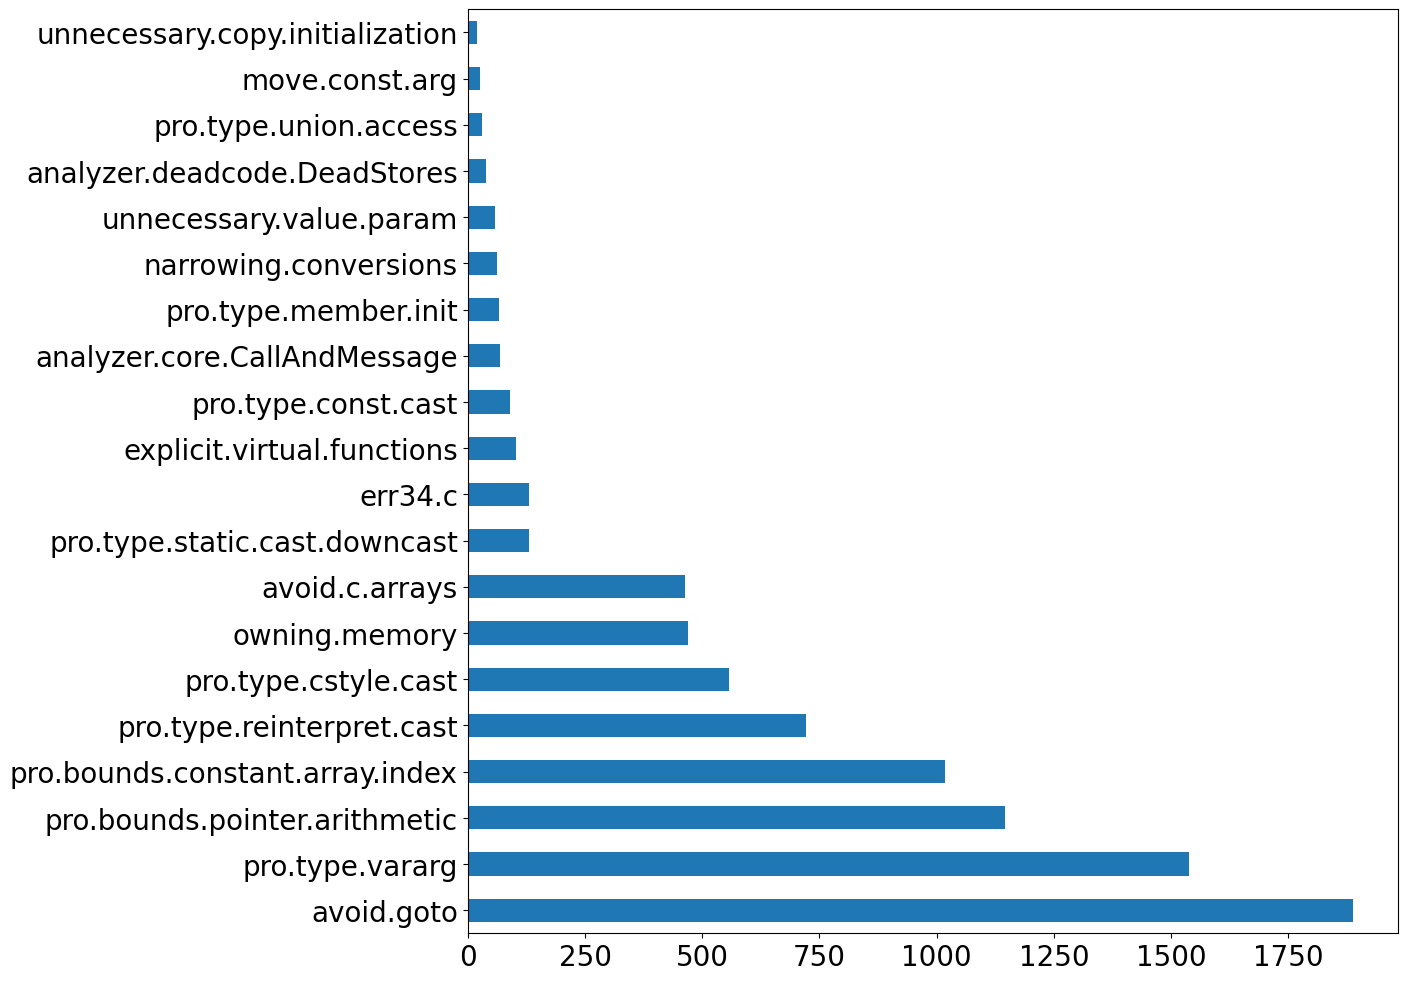
\includegraphics[scale=0.25]{./src/brls/brls_type.png}
		\caption{Most important bug-related alert types}\label{}
	\end{subfigure}
	\caption{Bug-related alert distribution}
	\label{results:bralerts}
\end{figure}

\begin{table}[H]
	\caption{Comparison against random ranking for the Bug-Related lines approach}
	\label{results:ranking_brls}
	\centering
	\begin{tabular}{@{}cccc@{}}
		\toprule
		& \textbf{S(R) metric}  & \textbf{Average FP to TP} & \textbf{Number Actionable} \\ \midrule
		\textit{Better than random Top 100 alerts}  & 1000 out of 1000 runs & 1000 out of 1000          & 50\% more than random      \\
		\textit{Better than random Top 1000 alerts} & 1000 out of 1000 runs & 1000 out of 1000          & 39\% more than random      \\
		\textit{Better than random All alerts}      & 10 out of 10 runs     & 10 out of 10              &                            \\ \bottomrule
	\end{tabular}
\end{table}

\begin{figure}[H]
	\begin{subfigure}{.5\textwidth}
		\centering
		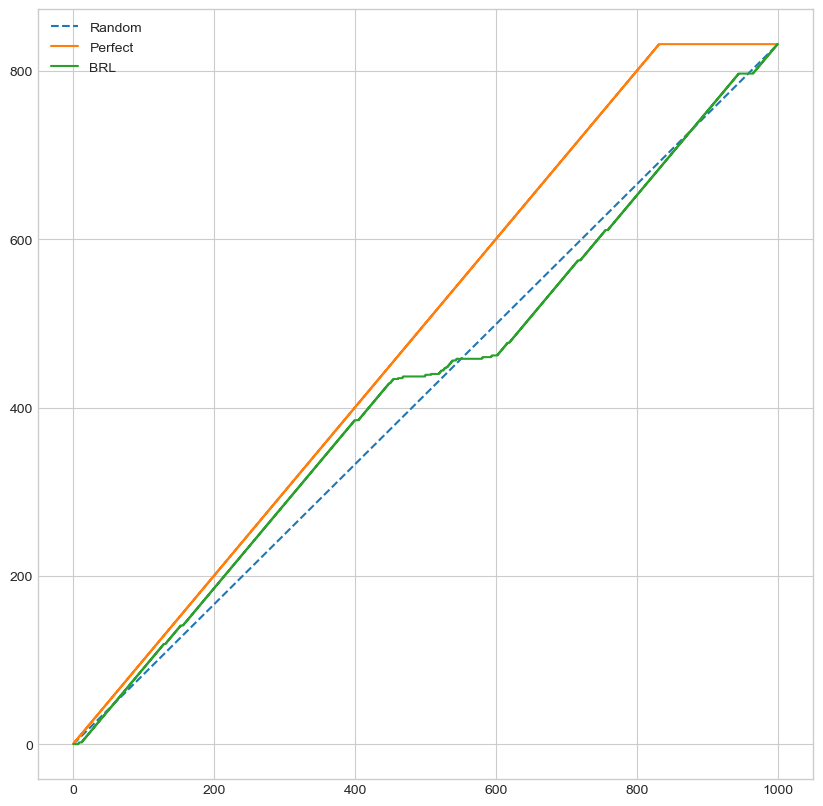
\includegraphics[scale=0.3]{./src/brls/brls_cumulative_graph_top1000.png}
		\caption{Top 1000 alerts}\label{}
	\end{subfigure}%
	\begin{subfigure}{.5\textwidth}
		\centering
		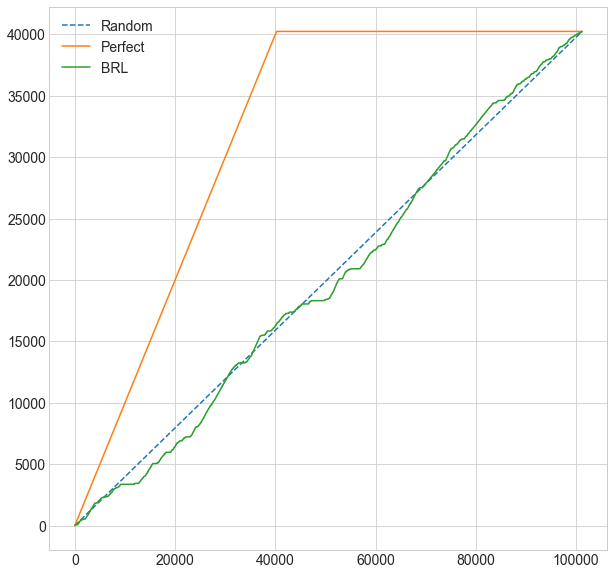
\includegraphics[scale=0.3]{./src/brls/brls_cumulative_graph_all.png}
		\caption{All alerts}\label{}
	\end{subfigure}
	\caption{Cumulative ranking graph for Bug-Related Lines}
	\label{results:cumulative_brls}
\end{figure}


\subsection{Combined approach}
\label{results:ensemble_approach}
One of the goals of this thesis was to explore the possibility of combing different methods that cover each others weaknesses in order to achieve a better ranking. The four evaluated approaches can be split in two categories: those that try to detect actionable alerts and rank them higher (\cref{method:fbrank}, \cref{method:actalerts}) and those that try to promote alerts that can potentially discover/prevent bugs (\cref{method:brls}, \cref{method:bugprediction}).

By analyzing the performance of the Actionable Alerts method (\cref{method:actalerts}), we see that there is not much room for improvement, since it is able to achieve great results for all four alert categories (see \cref{results:individual_categories}).

\begin{table}[H]
	\centering
	\caption{Classification metrics of Actionable Alerts method for individual categories}
	\label{results:individual_categories}
	\begin{tabular}{@{}ccccccc@{}}
		\toprule
		& \textbf{Precision} & \textbf{Recall} & \textbf{Specificity} & \textbf{F1-Score} & \textbf{Geometric} & \textbf{IBA} \\ \midrule
		\textit{cppcoreguidelines} & 97\%               & 97\%            & 98\%                 & 97\%              & 98\%               & 95\%         \\
		\textit{performance}       & 98\%               & 98\%            & 99\%                 & 98\%              & 99\%               & 97\%         \\
		\textit{clang}             & 98\%               & 98\%            & 98\%                 & 98\%              & 98\%               & 96\%         \\
		\textit{cert}              & 99\%               & 99\%            & 98\%                 & 99\%              & 99\%               & 97\%         \\ \bottomrule
	\end{tabular}
\end{table}


On the other side, if we look at the number of collected bug-related alerts (those that are located on bug-related methods on the first analyzed revision), we notice that it not even 5\% of the total amount of alerts. 
\henrique{Here you should also provide the numbers so that the reviewer can verify it is 5\%.}
Also almost all of them disappear with time, and can thus be considered actionable. There is in this case a big overlap in the training set of both the Actionable Alerts and Bug-Related Lines method, and since the first performs quite well, a combination is redundant. \henrique{Do you understand you just "shot yourself in the foot" here. If they are redundant, why did you do it? How can you justify your research? Maybe you should rewrite and tone down the statement.}

Also there is no clear correlation between a method being buggy and the actionable alerts that it contained (\cref{results:buggy_correlationss}). That is something that can be explained by bugs belonging to two categories: generic bug patterns (that can be discovered by static analysis) and domain specific bugs (difficult to detect by static analysis), as described by Habib et al. \cite{how_many_bugs}.

Nevertheless, acting on SA alerts will improve code quality which may lead to a decreased manifestation of future bugs in the methods that are considered as bug-prone.

Given the aforementioned considerations, a logical combination is a weighted Actionable Alerts method. The probability of an alert being actionable can be weighted by the probability of the method where it is located being buggy. That can also be augmented with relative weights for the alert types of bug-related methods (calculated by diving the number of alerts for each type by the total number of bug-related alerts).

The three inputs used in the combined approach are:
\begin{itemize}
	\item Probability of an alert being actionable.
	\item Probability of the method, where the alert is located, being buggy.
	\item Weights of alert types calculated as: $\frac{\#alerts \, of \, type_X}{\# \, of \, bugRelated \, alerts}$ for each alert type.
\end{itemize}

The problem of finding an optimal approach to such a combination can be defined as a \textit{multi-objective optimization problem}. We have the following ensemble ranking algorithm for alerts:
\begin{gather*}
Alert_{score} = w_{1} * Actionable + w_{2} * Buggy + w_{3} * AlertType
\end{gather*}

We want to find the optimal weights such as: we have the highest possible amount of actionable alerts at the top \textit{X} places, that also point to bug-prone methods.

By merging the different dataset, we can construct an ensemble test set for evaluating our approach. On this set, we have around 370 actionable alerts that also point to buggy methods. Since our classifiers are not perfect (especially the bug prediction one), we cannot expect to have all of them on the top of the ranked list.

We define the \textit{objectives} of the problem as:
\begin{itemize}
	\item Optimize the number of actionable alerts in the first 200 places.
	\item Optimize the number of alerts that point to bug-prone methods in the first 200 places.
\end{itemize}

We can also define \textit{constraints}, such as: there are at least 180 actionable alerts in the top 200 places.

To solve the problem we use the python \textit{Platypus} library \cite{platypus}. \henrique{And what technique is this library using? Bayesian network?}

As we can see from the results in \cref{results:ensemble_ranking} and \cref{results:ensemble_act}, we have an improvement in the ensemble method, regarding the number of bug-prone alerts in the top 200 and 1000 places. That does come with a cost, as beyond those first 200 places, the performance starts to heavily degrade (\cref{results:ensemble_act}). That should not be a big problem, since in practice it is rare to inspect that many alerts in one time. Also, with some fine tuning of the optimization problem, better results can be achieved. \henrique{How can you be sure that fine tunning can achieve better results? Do you have evidence to back that up? How much better?}


\begin{table}[H]
	\centering
	\caption{Actionable and bug-prone alerts in ensemble ranking}
	\label{results:ensemble_ranking}
	\begin{tabular}{@{}ccccc@{}}
		\toprule
		& \textbf{\begin{tabular}[c]{@{}c@{}}Actionable\\ Ensemble\end{tabular}} & \textbf{\begin{tabular}[c]{@{}c@{}}Actionable\\ Normal\end{tabular}} & \textbf{\begin{tabular}[c]{@{}c@{}}Bug-prone\\ Ensemble\end{tabular}} & \textbf{\begin{tabular}[c]{@{}c@{}}Bug-prone\\ Normal\end{tabular}} \\ \midrule
		\textit{Top 200 alerts}  & 185                                                                    & 200                                                                  & 187                                                                   & 137                                                                 \\
		\textit{Top 1000 alerts} & 265                                                                    & 1000                                                                 & 948                                                                   & 736                                                                 \\ \bottomrule
	\end{tabular}
\end{table}

\begin{figure}[H]
	\begin{subfigure}{.5\textwidth}
		\centering
		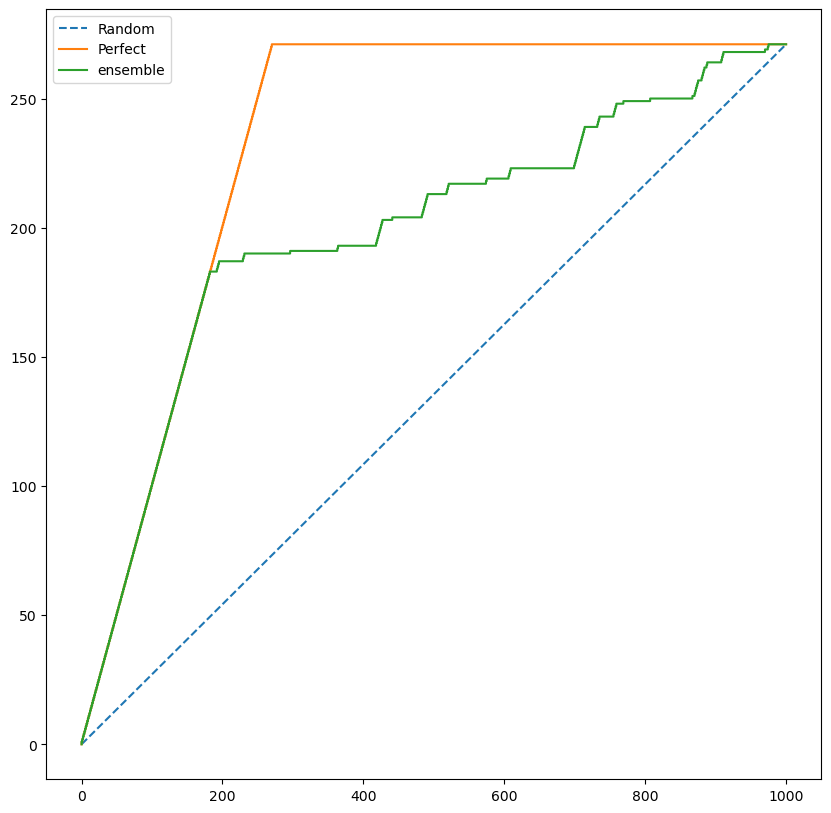
\includegraphics[scale=0.3]{./src/ensemble/ensemble_cumulative_graph_top1000.png}
		\caption{Ensemble method}\label{}
	\end{subfigure}%
	\begin{subfigure}{.5\textwidth}
		\centering
		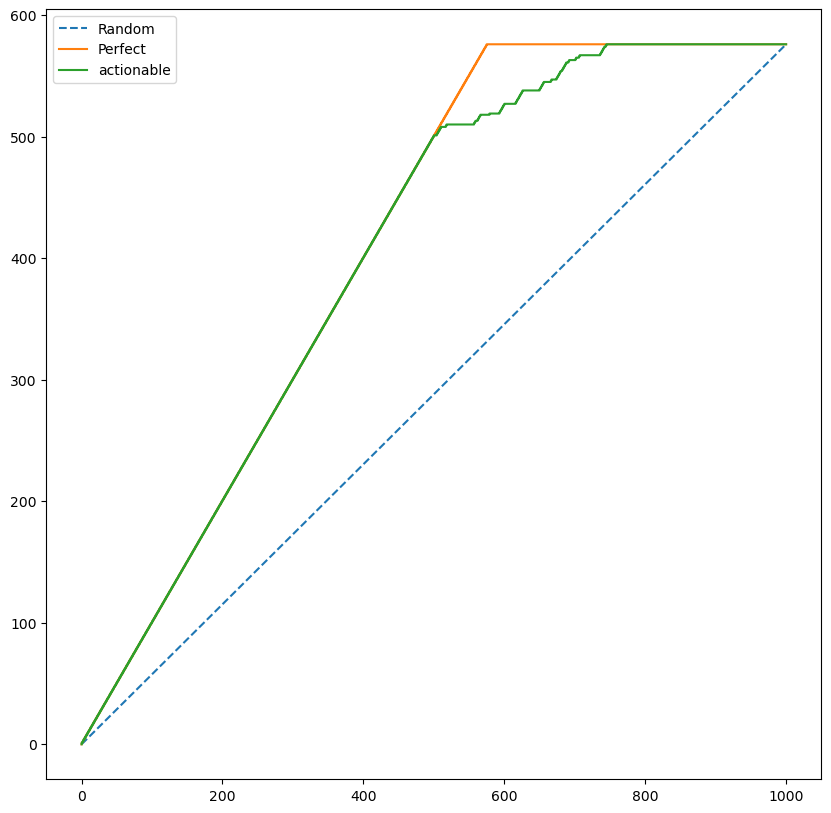
\includegraphics[scale=0.3]{./src/ensemble/actionable_cumulative_graph_top1000.png}
		\caption{Actionable Alerts method}
	\end{subfigure}
	\caption{Cumulative ranking graph for first 1000 actionable alerts}
	\label{results:ensemble_act}
\end{figure}

\begin{figure}[H]
	\begin{subfigure}{.5\textwidth}
		\centering
		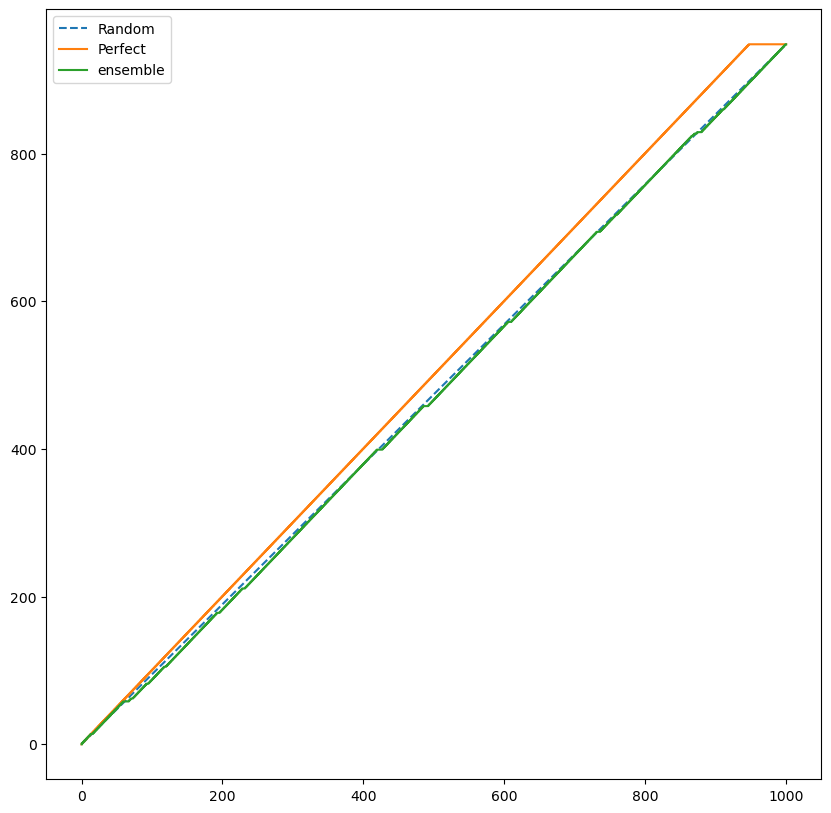
\includegraphics[scale=0.3]{./src/ensemble/ensemble_buggy_cumulative_graph_top1000.png}
		\caption{Ensemble method}\label{}
	\end{subfigure}%
	\begin{subfigure}{.5\textwidth}
		\centering
		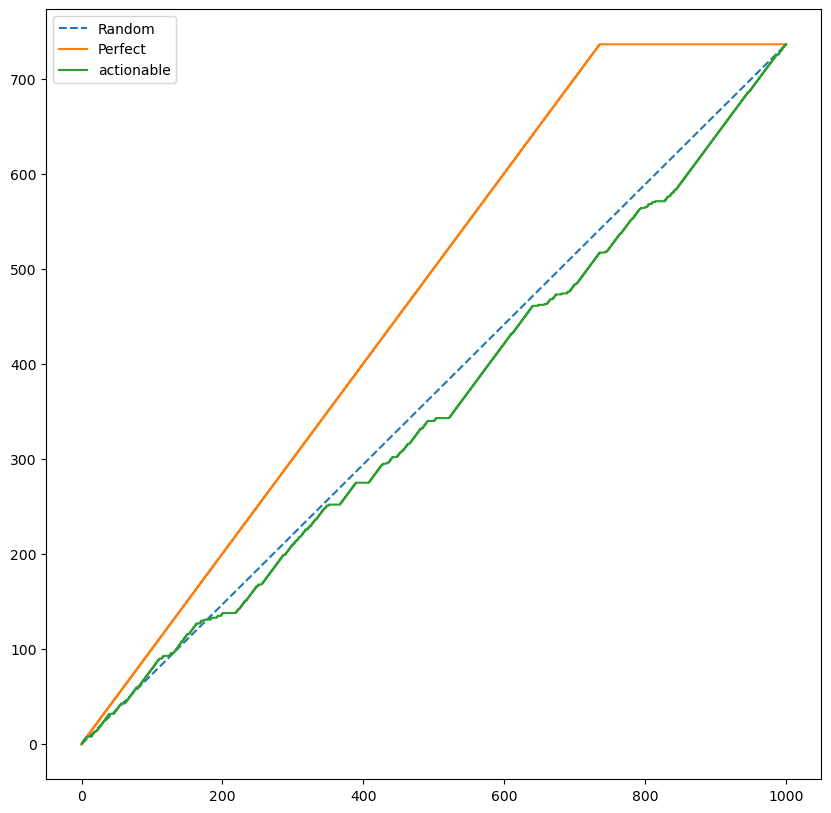
\includegraphics[scale=0.3]{./src/ensemble/actionable_buggy_cumulative_graph_top1000.png}
		\caption{Actionable Alerts method}
	\end{subfigure}
	\caption{Cumulative ranking graph for first 1000 bug-prone alerts}
	\label{results:ensemble_bugprone}
\end{figure}

%\begin{itemize}
%	\item There are at least 180 actionable alerts in the top 200 places.
%	\item There are at least 180 alerts that point to buggy methods in the top 200 places.
%\end{itemize}

